\documentclass[pageno]{jpaper}

% Change to current semester and year, e.g.:
% \newcommand{\IWreport}{Spring 2020}
\newcommand{\IWreport}{ 2020}
\newcommand{\quotes}[1]{``#1''}


\widowpenalty=9999

\usepackage[normalem]{ulem}

\begin{document}

\title{
The Automated Economist:\\ Using NLP to process Econometric Queries\\
Version Draftv1}

\author{Gabriel Stengel \\Adviser: Jaswinder Singh}

\date{}
\maketitle

\thispagestyle{empty}
\doublespacing

\section{Introdution }

Tabular data can be incredibly difficult to work with and analyze. Additionally many types of econometric and financial analysis require the use of sophisticated, expensive statistical tools such as Stata. For example, all Princeton upperclassmen must use computers in Firestone library that are preloaded with Stata for their independent work. Unfortunately, many students receive no formal training in Stata and are left handicapped when working inside the arcane enviorment. Using our new software,  users with or without requisite training in economics and statistics should be able to use their data efficiently: quickly finding and graphing interesting insights. Additionally, the chat-box like interface will allow even non-tech-savy users to analyze and augment data using natural language queries. Users themselves will contribute to the strength of our software with their every use. All previous queries are stored in an online database that can learn from human-queries. Also, because the software will be publicly available on github, economists and students can easily augment the software's capabilities by adding their own data analysis methods written in python. 

\subsection{Motivation}

Our software improves on conventional dataset analysis in two complementary ways. First, the user’s line of questioning can be open-ended. (Rather than hand-selecting variables and then using a computer to analyze a hand-selected economic relationship between them, she can use the toolkit to assist both her choice of variables and her choice of economic relationship.) Second, the manner of questioning is itself more flexible, in that it permits natural language inquiry. It will not require specific programming syntax. The end result is that users of the final product need not be well-practiced statistical coders. One could do serious and mature economic data analysis with no programming, Stata, or excel experience and only basic knowledge of the statistical tools customarily used by empirical economists.
Additionally, the project should prove fruitful outside of the fairly niche domain of academic, economic analysis. The work should lay the groundwork for a general purpose Question-Answering system that allows anyone to perform basic machine learning analysis on any dataset. NLP question answering on tabular data is a studied field, but by baking in greater statistical domain knowledge I hope to augment the usefulness of such systems.
\\
Moreover, there is a  plethora of tabular data available online by public and private organizations. Using and querying this data, however, is not easy. Ultimately, we imagine our tool could be built into online hosted data so that anyone with the goal of learning from online datasets can more easily search, manipulate, and analyze it.

\section{Problem Background }

The crux of our software boils down to two problems: (1) the problem of interpreting natural language queries, and (2) the problem of reasoning about unseen data and automating advanced economic insights. How can we parse and understand high-level statistical queries? And, how can our engine find interesting statistical insights that humans might not be able to (even given good working knoledge of tools like Stata).  Fortunately, there is a large body of NLP research into question modelling and parsing that our software can capitalize on. And, there is also a corpus of economic research on automating economic anaysis. \\

Attempting to answer natural language queries on semi-structured tables is complicated for a number of reasons. First, there is an open-ended set of relationships between datums and columns, and second there are exponential possibilities for the logical forms that statistical questions can take. \\
However, there is a great deal of research done on natural language retrieval tasks using tabular data, although these queries differ greatly to ours in scope and complexity, the results and methodologies heavily informed our software design. Additionally, lots of research has been conducted by economists on automating statistical insights into economic data. 

\begin{figure}[!hbt]
\centering
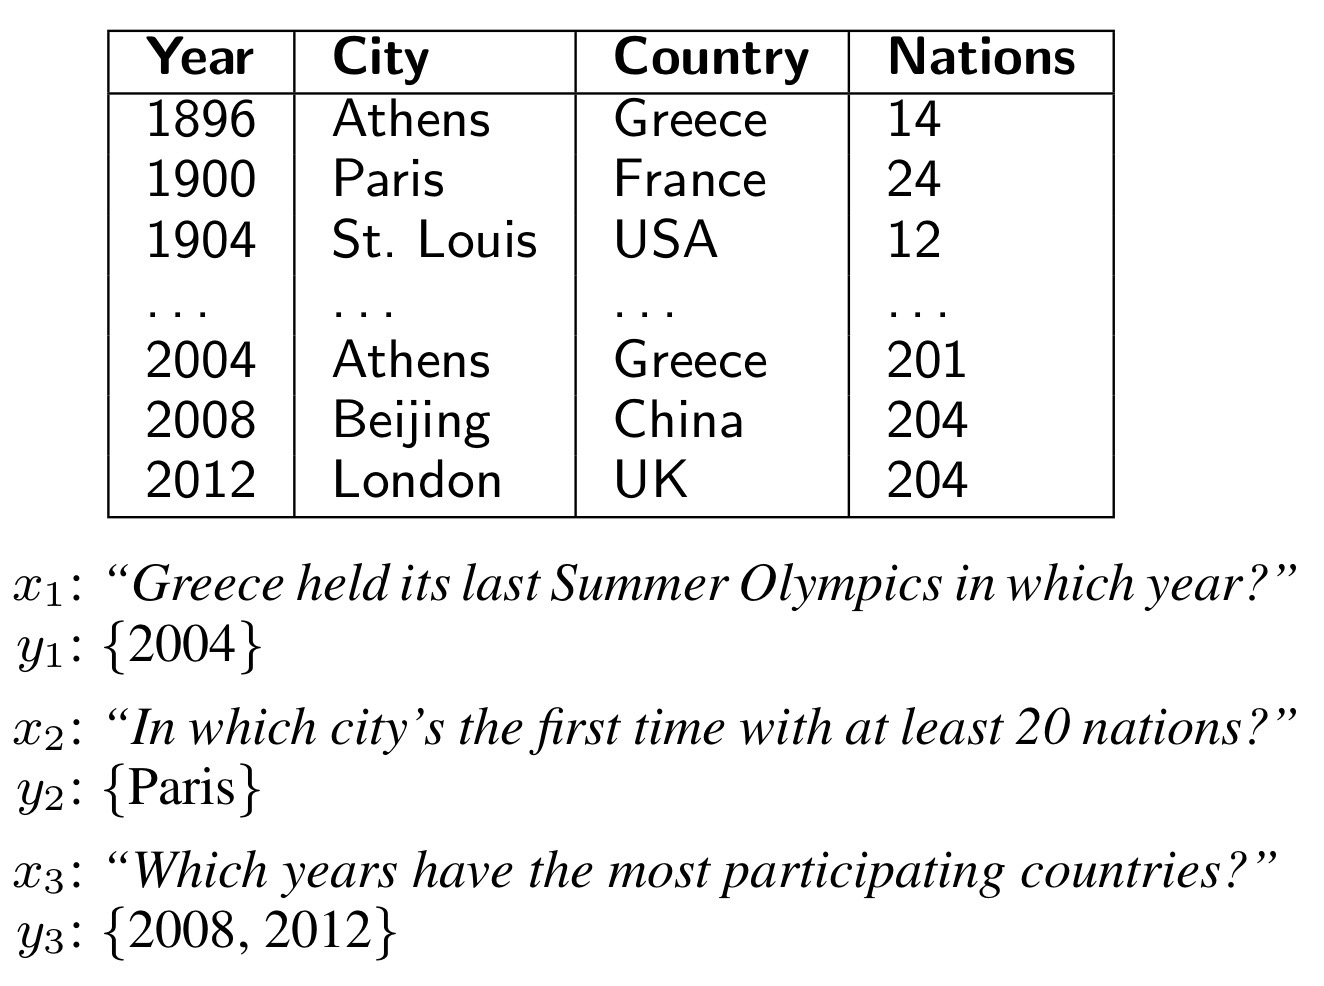
\includegraphics[width=0.75\linewidth]{imgs/comp_semantic_parsing.jpeg}
\caption{Example of data retrieval queries.}
\label{fig:retri}
\end{figure}

Figure \ref{fig:retri} shows an example of previous research that has achieved $76.1\%$ accuracy (the highest existing baseline for these types of queries). 


\subsection{Previous Work }
Here is a list of previous publications in the field of tabular question answering and economic data anaylsis that have influenced our work.
\begin{enumerate}
	\item   \href{https://doi.org/10.3115/v1/P15-1142} {“Compositional Semantic Parsing on Semi-
Structured Tables.”}
	\begin{itemize}
		\item  Pasupat and Liang of Stanford discuss methodology for algorithmic processing of natural
language in dataset analysis. They suggest “knowledge graphs” that bind and process logical forms of queries. The authors use and provide a “Wiki Table Questions” for model training and outline floating parsing algorithms and pruning choices for a set of problems very similar to ours. Our software makes use of similar knowledge graphs and logical parsing of questions, however the domain of queries is slightly different.  \\
	\end{itemize}
	\item  \href{http://ceur-ws.org/Vol-2044/paper1/paper1.html}{“TableQA: Question Answering on
Tabular Data.”} 
	\begin{itemize}
		\item Vakulenko and Savenkov examine a similar set of problems – still related to processing natural language queries in dataset analysis situations. They write about deep learning and neural network approaches, using end-to-end memory networks architecture. However, their results are suboptimal, and due to the limited amount of data we would have for training our own networks, we have stayed away from deep learning approaches.\\
	\end{itemize}
	\item \href{ jstatsoft.org}{“Tidy Data.”}
	\begin{itemize}
		\item Wickham writes about the uses and conventions of “tidy data,” a standardized way of formatting data that aims to lessen the “huge amount of effort [that] is spent cleaning data to get it ready for analysis.” Data is tidy if 1) every variable forms a column; 2) every observation forms a row; 3) every type of observational unit forms a table. We plan to ask our users to put their data in tidy form so there is less plumbing on our end to deal with the hairy problem of variable identification.\\
	\end{itemize}
	\item \href{https://doi.org/10.1017/S0266466605050024}{“Automated Discovery in Econometrics.”} 
	\begin{itemize}
		\item Phillips comments on the state and future of automated discovery in economic statistical querying. He writes that his “experience with automated discovery algorithms in econometrics leads me to believe that these methods will play an important role in the future use of applied econometrics.” Pointing to a growing practical research agenda – as policy decisions become increasingly driven by empirical relationships – he sees a great degree of under-realized potential in this sort of automation.\\
	\end{itemize}
	\item  \href{https://doi.org/10.1162/001152604772746710}{“The Automation of Discovery.”} 
	\begin{itemize}
		\item Like Phillips, Clark writes excitedly about the future of automated model selection in science. He points to a few examples from the late twentieth century in which the power of computing helped define important variable relationships. And he sees great promise in machines’ potential to grow their influence and further assist in empirical research. He goes so far as to compare traditional research methods to searching for needles in a haystack and automated model selection methods to “[running] a magnet through the haystack.”\\
	\end{itemize}
	\item \href{https://doi.org/10.1177/0049124103260341}{“Automating the Selection of Model-
Implied Instrumental Variables.”} 
	\begin{itemize}
		\item Bollen appears to be the eminent scholar on automated instrument selection. He suggests a maximum likelihood technique for selecting variables for 2SLS analysis.\\
	\end{itemize}
\end{enumerate}
 
Add this guy: https://arxiv.org/abs/1710.07032\\
and
https://www.cs.toronto.edu/~muuo/writing/semantic-parsing-in-your-browser/ and
\\
https://arxiv.org/pdf/1809.08887v5.pdf and \\
https://arxiv.org/pdf/1810.02720v1.pdf and
\\ https://medium.com/@tao.yu/awesome-sequence-to-sql-and-semantic-parsing-1d7656861679 \\
\href{https://www.annualreviews.org/doi/pdf/10.1146/annurev-linguist-030514-125312}{Liang and Potts 2015}.
 
\section{History of The Problem}

SHRDLU (Winograd 1972)
Domain is geometric objects .
Much easier because it was a really constrained domain and world.

CHAT-80
Hand built grammer and lexicon.
Similar, small domain on geographic data.

Show examples:
"Which country berdering the Mediterranean borders a country that is bordered by a country whose population exceeds the population of India?"
...
Answers.. impressive but very complicated.

However, the allowable phrasing of questions is limited because it is hand written. Slight changes and the system cannot handle it.

 Problem is the tradeoff between robustness and precision: i.e. domain and accuracy... Part of what we wanted to do in innovation, was create a dialogue between machine and person so that the machine can augment its understanding through a back and forth. Not ambitious enough to create a fool proof system that can interpret large statistical queries from a large domain with  impeccable accuracy.
 
 Since our problem is not database querying, there is not that much similar research. The problem of querying databases is certainly relevant to our project, howver they are slightly different scopes. 

\section{Semantic Parsing}
The crux of our paper. Understanding the natural language queries and parsing them into their logical forms.

Part of NLU - Natural Language Understanding. 

First we parse every sentence into one of two things:  "Chat" or "Commands". Commands are ...

All queries are things that could be done with an economic library and python. 


Challenges of Semantic Parsing:
1. Scope ambiguity. Groucho marks joke: A woman gives birth in the United States every 10 seconds. Stop her!... Ambiguity... in commands. Different logical consequences. How do we decipher these ambiguities: multiple options... restrict domain (i.e. add more rules to input?)? Train predictors? Assign likelihood scores to logical predictions. 

We are aided by the fact that a lot of constraints for our problem are limited by our domain: (econometric and data anaylsis).


Think about the following ambiguities:
A) What is the mean of ..
,..
..


Goal of Semantic Parsing:
Translate natural language into a \textit{formal meaning representation} on which a machine can act.* (definition from stanford nlp lectures). We start by choosing a target output representation.

If this were pure database exploration and simple anaysis. Examples would be something like translating into a procedural language. Or for voice commands you would use something like "intents and arguements" (high level intents).  We would output into something like sql, that allows database queries. ...

However our product has a diferent goal. So we went with a different end goal.

Looked at two different leaping off points:
1. SEMPRE
2. SippyCup:
Commonly used at google and apple but "simplified"
Sippy cup units:
1: natural langauge artihmatic...2..3. geographical queries (modern approach to chat 80)

Similair to SEMPRE, but in python and with less training. Up to date in the field.

-Defining possible syntactic structures using context free grammar (CFG)\\
- Construct semantics bottom up, following syntacic stracture\\
- Score parses with a log-linear model learned from training data \\
- phrase annotators for recognizing names, numbers, places, times etc \\
-grammar induction to avoid manual grammar engineering \\

CFG (Context Free Grammar) has two parts.\\

\textbf{Syntactic part and semantic part} \\
Syntactic -- fairly conventional. Usually not deterministic, many possible deviatins per input. Normal for naturalk language utterances, because they are usually ambiguous (even for native speakers).

Terminals and non terminals. ... Use an example: \$LOC -> Google
 ..
 
 PArsing Algorithm:
 generate all possible parses using dynamic programming: CYK chart parsing algorithm \\
 rewrite the grammar rules so that they are all binary or unary so that we only have to think about splitting parses in two rather than 3,4, or 5.\\
 (Maybe use beam search)\\
 NOW, semantic attachments to CFG rules: outpute which are fragments of our meaning representation.\\
 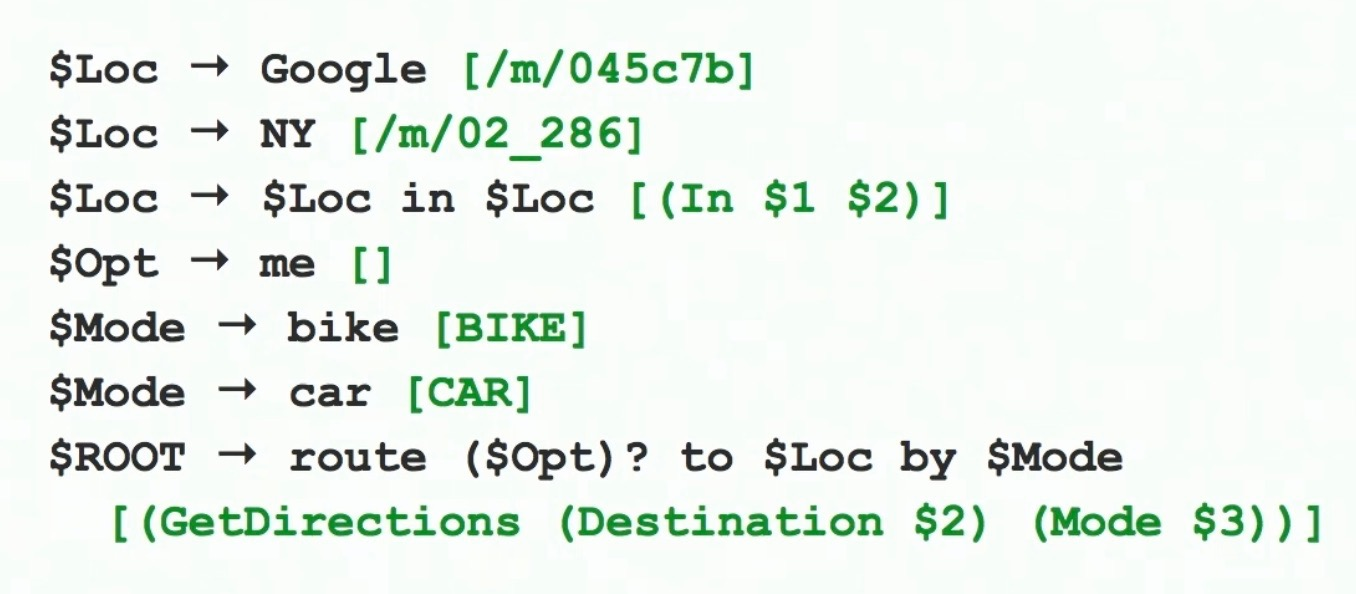
\includegraphics[scale=.28]{imgs/sem_attach.jpeg}
\\
Can see the google is just an ID, for the location you can see its a method to build up a new location (fragment of meaning representation).
So this is a full example parse:
(include an example or image)...
Happens bottom up. Because its far more efficient for natural language, top down is prohibitively expensive. Bottom up allows you to eliminate unlikely possibilities early in the process. Even very pedestrian inputs have thousands of possible parses, you must prune them to make sure you have only a finite list of highest possibilities (beam search).
\\
Use \textbf{Annotators}:
Don't want a million rules recognizing things like NY, New York, Big Apple... 
\\
instead leverage intelligence of special purpose annotators (using a database like freebase in our case). (FreebaseAnnotator, ContactAnnotator, DateAnnotator)... special black box models that run over the input query and generate hypothesis about how to interpret small spans and input them into the syntactic machinery. Running the annotator first helps to limit the number of possible parses.  \\

\subsection{Problem of ambiguity}
When grammar supports multiple interpretations, how do you choose one? \\ 
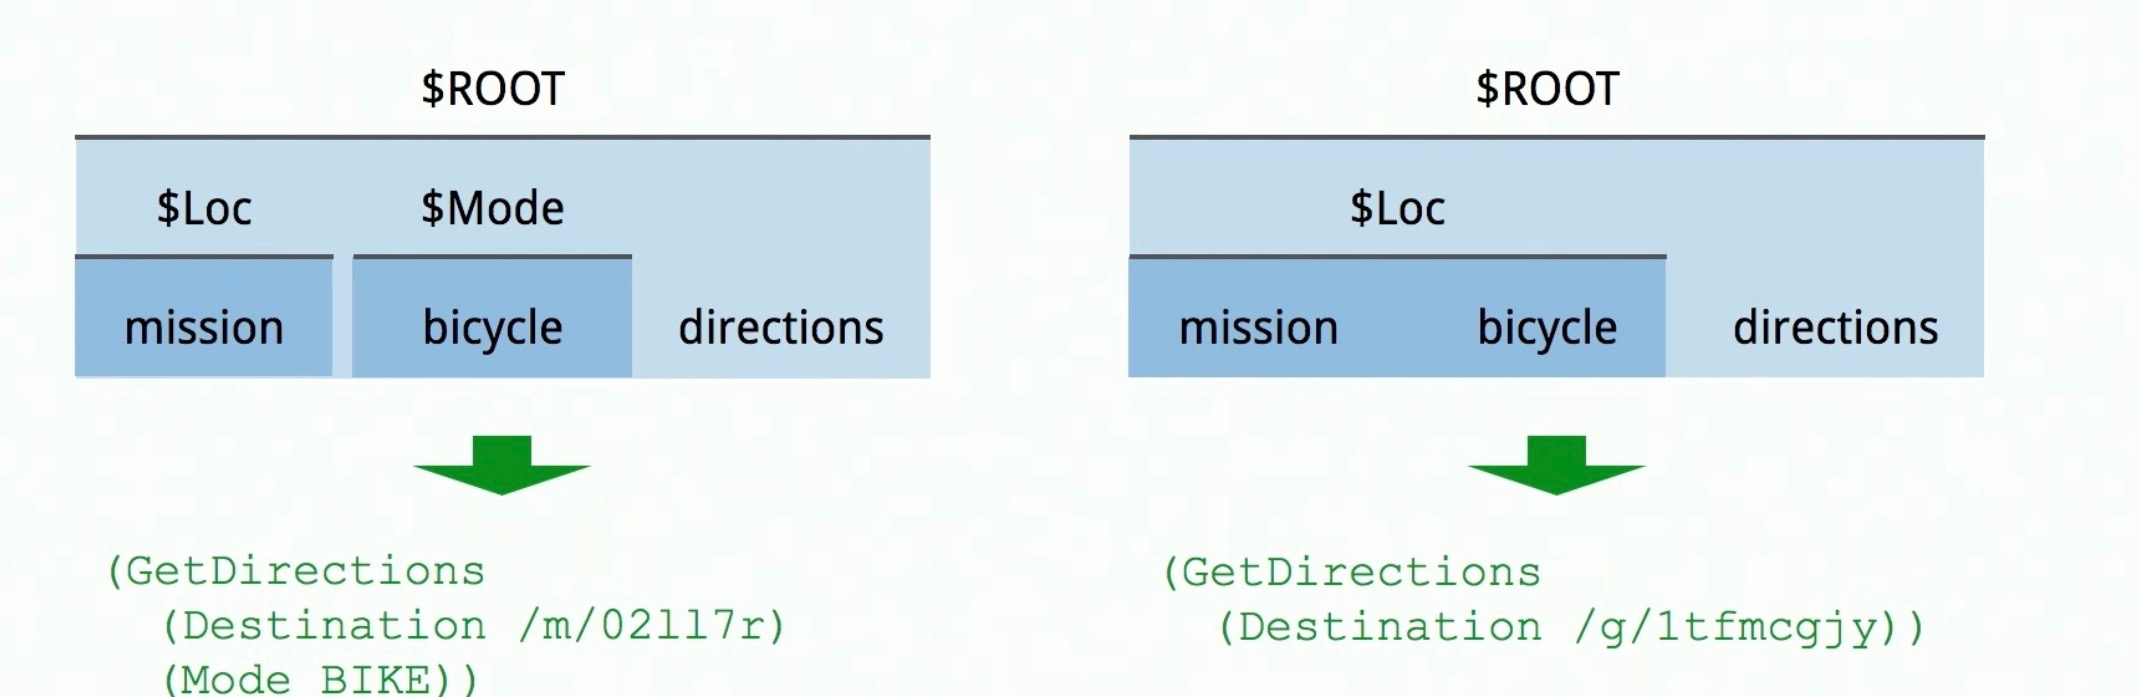
\includegraphics[scale=.2]{imgs/ambig.jpeg}\\
Change this example to a method name and a column name that could be ambiguous.

So how do we deal with this ambiguoity, because having two parses is most likely a best case, and its more likely that an input query has hundreds if not thousands of possible parses?

We score the parsed phrases.

\subsection{Scoring model}
Use a log-linear model to score alternative derivations. (parses) 
Features from input $\textbf{X}$, semantic yield $\textbf{y}$, and derivation $\textbf{z}$. 
So we build an assortment of features from the input... 
examples of features: indicator function that shows co-occurence of the word "calculate" and "mean". Weak features\.
or boolean features that mark specific CFG rules or categories (because some rules in the grammar might be more or less likely to be in a query, think of good example. ) Or a feature representing the confidence of the annotator (how confident it is that New York City is a city for example).

So we just take the dot product of features and weights, and then use soft max to turn it into a probability.

Where do we get the weight vector theta? We estimate them using training data and EM-training. Expectation Maximization. Alternates between E and M steps. In E: use current model parameters to parse the training inputs in our data. M step: change the weights of the model to put more probability mass on the n-best list that actually generated the correct target semantics. And repeat. 

\subsection{Grammar Rules}
So where do our grammar rules come from? if it were a small domain, grammars with a few dozen/hundred rules are enough. At that scale you manually generate and write the rules by looking at example queries. However, large domains don't work for this. The domain is too large and complex, needing thousands of rules to model the domain well. Not feasible to write them manually, instead we want to learn them from training data. Instead we want to use grammar induction. 

For our project we took a mix of both, but we assume that the more use our program gets the more grammar induction we will be able to do.

Some strategies: generating all possible rules, but there is an exponential blow up and so this is a little too computationally expensive. We need to keep the size of the grammar manageable. 




\subsection{Uses Of Training Data}:
To induce rules of the query grammar. Which syntactic productions should be part of the model. The other way of using the data is to estimate the parameters of our scoring model. This works hand in hand. Underscores the importance of data. Ideally we need LOTS and LOTS of data. To do this at scale you have to invest a lot of money in human annotators. Google fb etc use things like the mechanichal turk to annotate data. However this is very expensive, so instead we want to try two different things:
Learn from indirect supervision (learning from denotations -- having human annotators produce the answer rather than the logical forms) and learn on the job (online learning).

Learning from denotations is pretty important... learn from the answer rather than the logical form. A little harder in our case because our answers are not simple nouns, they are advanced statistics.

Cite - "The Unreasonable Effectiveness of Data" - 2009. 


\section{Review of A Survery on Semantic Parsing}
"A significant amount of information in today's world is stored in structured and semi-structured knowledge bases. Efficient and simple methods to query them are essential and must not be restricted to only those who have expertise in formal query languages. the field of semantic parsing deals with converting natural language utterances to logical forms that can easily be executed on a knowledge base."

Intersection of NLP, information retrieval, and human computer interaction. 

Mapping from natural language utterances to meaning representations. To the point where the machine can perform automated reasoning. 

HOW ITS DIFFERENT FROM SEQUENTIAL TASKS: like a chatbox or text generation:
"It is worthwhile to recognize that semantic parsing is inherently different from other sequential prediction tasks such as machine translation and natural language generation in that unlike the latter, it involves prediction of inherently structured objects that are more tree like. Additionally, it has to also adhere to certain constraints in order to actually execute in a given environment, introducing unique challenges."


\begin{enumerate}
\item Query: "What is the correlation between entertainment spending and age?"
\item Context: The dataset.
\item Program: (CALL correlation ON (enterq AND age))
\item Answer: Some pandas column
\item Grammar: Our custom made data query grammar
\end{enumerate}


"The mapping to logical forms typically relies heavily on the availability of annotated logical forms and difficulties in procuring such labeled data gave rise to attempts at using alternative methods of training involving weak supervision."

Meaning Representations (MR) are the same as "logical forms." They are the end goal of semantic parsing.


Overview of semantic parsing:\\
"Semantic parsers map natural language (NL) utterances into a semantic representation.
These representations are often (interchangeably) referred to as logical forms, meaning representations (MR) or programs (. The representations are typically executed against
an environment (or context) (e.g. a relational knowledge base) to yield a desired
output (e.g. answer to a question). The meaning representations are often based on an
underlying formalism or grammar . The grammar is used to derive valid logical
forms. A model is used to produce a distribution over these valid logical forms and a parser
searches for high scoring logical forms under this model. Finally, a learning algorithm
is applied to update the parameters of the model, by using the training examples"

We also assume that we have a deterministic executer: i.e. the statistical engine of Athena. That we can run as many times as is necessary.\\

When thinking about what sort of Meaning Representaion we wanted, we considred the three most popular languages for them:
\begin{enumerate}
\item \textbf{Logic Based Formalisms}: 
\item \textbf{Graph Based Formalizm}: based on the placement of edges/nodes etc. Easier for humans to comprehend and read, when compared to esoteric logic. Also lots of graph theory literature exists for processing graphs.
\item \textbf{Programming Lanugages}: its becoming more and more common to translate directly into a high-level language like Java, python, SQL and bash
\end{enumerate}
Our choice: ... .

\subsection{Grammar Design}
"When dealing with complex but well structured queries, strict grammar rules provide computational advantage by virtue of generating fewer possible derivations.... On the other hand, when the language is noisy, floating rules have the advantage of being able to capture ill formed sentences such as those produced when dealing with crowd sourced utterances." We experiment with both. And offer two models: one for stricter, with higher accuracy and one for lay people with worse accuracy.

\subsection{Underlying Context}
All MRs are with respect to an underlying context or environment from which they derive their meaning. Examples are, graphs, structured knowledge bases, tables spreadsheets, images and so on. For us we will use multiple contexts: freebase as well as the uploaded data.


\subsection{Problems}
"A consequence of the fact that these systems require complex annotation is that they are hard to scale and they only work in narrow domains. Generating the data sets using manual annotation is still a formidable task and due to this, supervision in various different forms has been explored. the next two sections list several of these attempts."

One possible solution: denotations, or training the system just on the \textbf{result} of the execution (rather than the full logical output in the formal meaning representation. This is \textbf{weak supervision} and it poses certain challenges. The first is a very large space of potential programs and executions that have to be explored, and the second is that  there are a number of "spurious programs" that would lead to the correct answer purely by luck.


\section{Choosing between CCG and CFG}
I dont really know lol. But should probably have a good reason...
\\


What Pasupat and Liang did: "To combat the issue with the unseen tables, their approach first builds a knowledge graph from the table in question resulting in an encoding of all the relevant relations. Using the information from this graph, candidat parses of the question are generated and these candidates are ranked using a log linear model, whose parameters are learned using MML."

--> We should also use a knoledge graph.

\subsection{Learning from User Feedback}:
Iyer et al 2017 use learnign from user feedback, binary feedback.


\subsection{What about RNNs}
Theres been an increase in Seq2Seq methods. Largely successful in machine translation. Has advantages like getting rid of intermediary stages of the parsing, but less able to capitalize on the built in domain logic and compositionality.

\subsection{Take Aways for us: What we do different:}
A 2019 comprehensive study of semantic parsing literature wrote that:
"Integrating confidence estimation in the responses from a semantic parser has been largely unsexplored and we believe is a useful direction to pursue. In order to have meaningful interactions with conversational agents, knowing when the model is uncertain in its predictions allows for adding human in the loop for query refinement and better user expierence." This is precisely what we're doing. By making this into a usable product rather than merely a research endeavor we have to incorporate these components. As a result our application is also interesting from the academic research perspecitve, as we take into account user feedback when training.\\

\section{SippyCup: Our baseline Semantic Parser}
Their approach:
\begin{itemize}
\item CFG with Semantic Attachments
\item Chart Parsing
\item log-linear feature based scoring
\item Learning Scoring parameters with Stochastic Gradient Descent
\item Small amount of grammar induction (perfect for our purposes where there isn't a large enough dataset to induce all grammar rules)
\end{itemize}
Diagram would be good:
\\ Linguistic input $\to$ Semantic Parser (deals with polysemy, ambiguity, indexicality... etc )$\to$ Meaning Representation $\to$ Executor $\to$ Result.

\section{Approach}
Using data: we will create a list of sample inputs and write their target outputs. Although this would be tedious and error prone with too many inputs without the use of a program like mechanichal turks, it is useful for helping start our parser. Another option would be just to write down the denotation for a query -- i.e. what the actual result should be, however for the complex econometric anaysis that we will be doing, it will be hard for a machine to learn parsing from just the denotation.\\ \\

Syntactic Parsing: \\
(Read up about Syntactic Parsing in \textit{Speech and Language Processing} by Jurafsky and Martin.\\
The goal is to create a tree structure over the inputs that represents its "constituency structure." The constituency structure is basically just how we group words into larger and larger phrases when thinking about the meaning of a sentence or text.  A great example about how this grouping affects meaning is found in the Stanford class lecture: \\

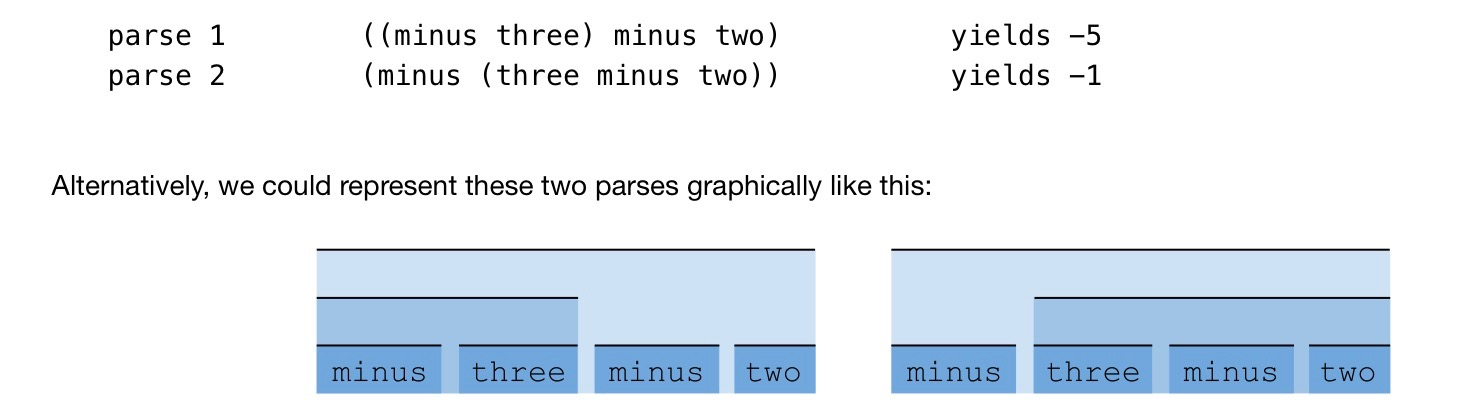
\includegraphics[scale=.2]{imgs/synt_amb.jpeg}

Next, we assign \textit{categories} to each word. This basically just means labeling words to let us know a little bit more about its purpose in a query. \\

\subsection{Chart Parsing}
How do we find the set of parses for the input which are allowed by our given grammar: the answer is using the CKY algorithm -- a dynamic programming chart parsing algorithm  (FIGURE OUT WHY WE'RE USING THIS ALGORITHM OPPOSED TO A DIFFERENT ONE). 

Using GRammar class, parse class etc...
Next comes semantics...
\subsection{Semantics}
We now look at lexical semantics: this is a bottom up composition.\\
We use the principle of compostionality (attributed to Gottlob Frege) for building up these semantics at each node.\\

\textit{The meaning of a compound expression is a function of the meanings of its parts and the manner of their combination}. (not sure if I can use this direct quote, find somewhere to cite).\\

This principle is the central pillar of Montague grammar, "which provides the theoretical foundation for much academic work in semantic parsing. 

We have semantic rules for how to build up the semantics from a given parse. Currently we "eagerly" build the semantics, i.e. we create the semantic representations as we parse the queryies.

\subsection{Scoring Candidates}
Use a log linear scoring function that is just the innerproduct of the features of the query and the weights. Leaves us with two difficult questions:
\begin{enumerate}
\item Feature Engineering: \\ defining features that will be most discriminating in judging good parses from bad
\item Weight Learning:\\deciding which features are most important
\end{enumerate}

One place to start with feature engineering is "rule features" -- recording the number of times a rule was used in a given parse. This is a basic feature often used in semantic parsing.  They are fairly effective in discriminating between good and bad parses. \\

We started by hard coding some features and then setting weights by hand. However as accumulate more and more training data, the strategy of setting features by hand based on domain knowledge seems less and less feasible. \\

Instead, we set up the infrastructuer for learnign using SGD (borrowed and worked from \href{https://www.annualreviews.org/doi/pdf/10.1146/annurev-linguist-030514-125312}{Liang and Potts 2015}. 


\subsection{Grammar Induction}


\section{Design Decisions}

\subsection{Designing a Meaning Representation}
We need a very specific meaning representation. One that works well for our needs, some properties should be:
\begin{enumerate}
\item Straight Forward
\item Un-ambiguous
\item Human Readable (for annotative purposes)
\item Machine Interpretative/Executable
\item Specific
\item Concise
\item Dynamic (able to be amended and changed based on back and forth)
\end{enumerate}

\subsection{SECONDARY APPROACH}
Instead of doing fully fleshed out semantic parsing, we also look at the possibility of doing intent recognition and NER (named entity recognition) -- a sort of simplified approach used in some applications like Siri and Alexa. 

This approach better serves things like travel queries -- domains that are far more diverse with much wider lexicons (where the size is potentially unbounded) and the words and phrases can be assembled in a far greater variety of ways. Also its more ambigous.  And inputs can be messier i.e. there are more spelling errors and grammatical typos when people use google then when they use stata. HOweveer, the good tradeoff: the meaning representaions / semantics of such systems are much simpler. Probably only needs to represent a few things, like the intent and the arguments: e.g. intent: directions Arguments: to: princeton from: new york.  
looks like:\\

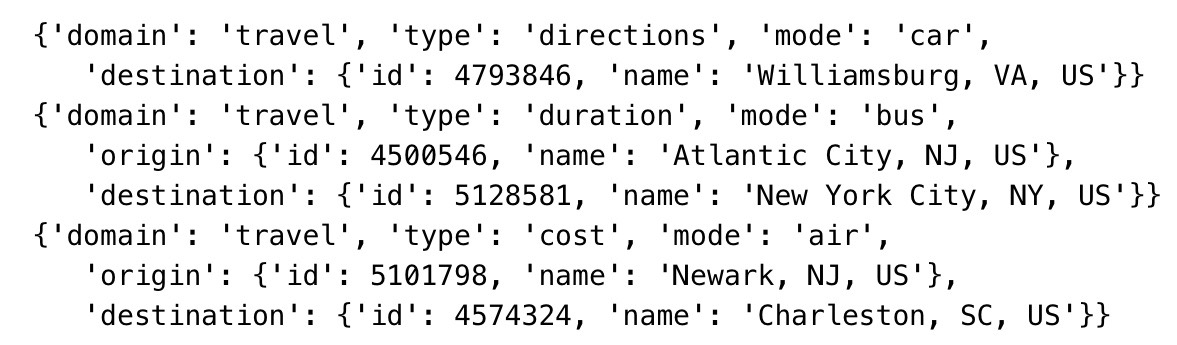
\includegraphics[scale=.25]{imgs/trav.jpeg}\\
So the semantic representation doesn't need deeply-nested recursive execution and logical form design.

\textbf{"The difficulty of producing annotated data, and the consequent paucity of such data has been the eternal bane of research in semantic parsing. Indeed overcoming this obstacle was the chief motivation for the shift made by Liang et all in 2011 to learn not from semantics but from denotations, which are easier and cheaper to generate via crowdsourcing. Despite this shift, annotated data remains scarse. To this day, the largest standard dataset for semantic parsing is WebQuestions dataset and contains only 5810 examples" -- Stanford} Manual denotation is time consuming and boring and thus expensive. 


\section{Deep Dive into Features of Our Grammar}
We don't enforce grammatical rules to be in Chomsky normal form, instead we just reform rules to obey the form in grammatical processing. Makes grammar engineering much easier, which is important because we are doing so much of it by hand.
\begin{itemize}
\item Annotators
\item N-ary lexical rules (i.e. (Rule('column': 'entertainment spending')
\item Unary Compositional Rules (very helpful but have to be weary of creating cycles where the number of possible parses is infinite.)
\begin{itemize}
\item One strategy for dealing with cycles is having an upper bound on the number of possivle parses. We tried this but think there are easier options (as in not creating grammars that allow for it).
\end{itemize}
\item N-ary Compositional Rules
\item Optional Elements
\item Designated start symbol
\end{itemize}

\subsection{Annotator}
IDea of annotator: instead of manually entering rules for all possible labels of something like "\$Function:" "average", "correlation" (which would be tedious and error-proce) we instead use annotators to do that on the fly. 

\subsection{Grammar Engineering}
Start with our training set. Keep adjusting and adding rules until our oracle accuracy is higher:

Oracle Accuracy: The proportion of examples for which the first pare is correct. This is normally thought of as an upper bound on accuracy. And the difference between oracle accuracy and normal accuracy reflect the scoring model's ability to find the correct parse among multiple candidates.
 An option fo rour grammar is a \textit{phrase bag grammar} -- where the phrases are more important than the order of said phrases. E.g.:
\begin{itemize}
\item Graph the  correlation of x and y 
\item Find the correlation of x and y and then graph it
\end{itemize}
Different orders, same intent, same phrases.
For us, the phrases could be of two types: \textbf{query methods} and \textbf{method arguments} \\

ACTUALLY IN PRACTICE:
After creating a database of limited scope -- functions with only a single arguemnent, we were able to get a denotation accuracy of $62\%$ with just moderate grammar engineering.


\subsection{Thought about using GraphKB as the structured knoledge base}
This is better served for things like look ups or searches or simple information-retrieval style questions.

\subsection{Evaluation Notes}
We want some queries that dont work and are not included in our domain because that will show us that our system WORKS!  

\subsection{Our Semantic Representation}



THIS STUFF SHOULDN'dsT BE IN FINAL THESIS. (below this statment)

\section{Thesis Draft Update}
\begin{figure}[!hbt]
\centering
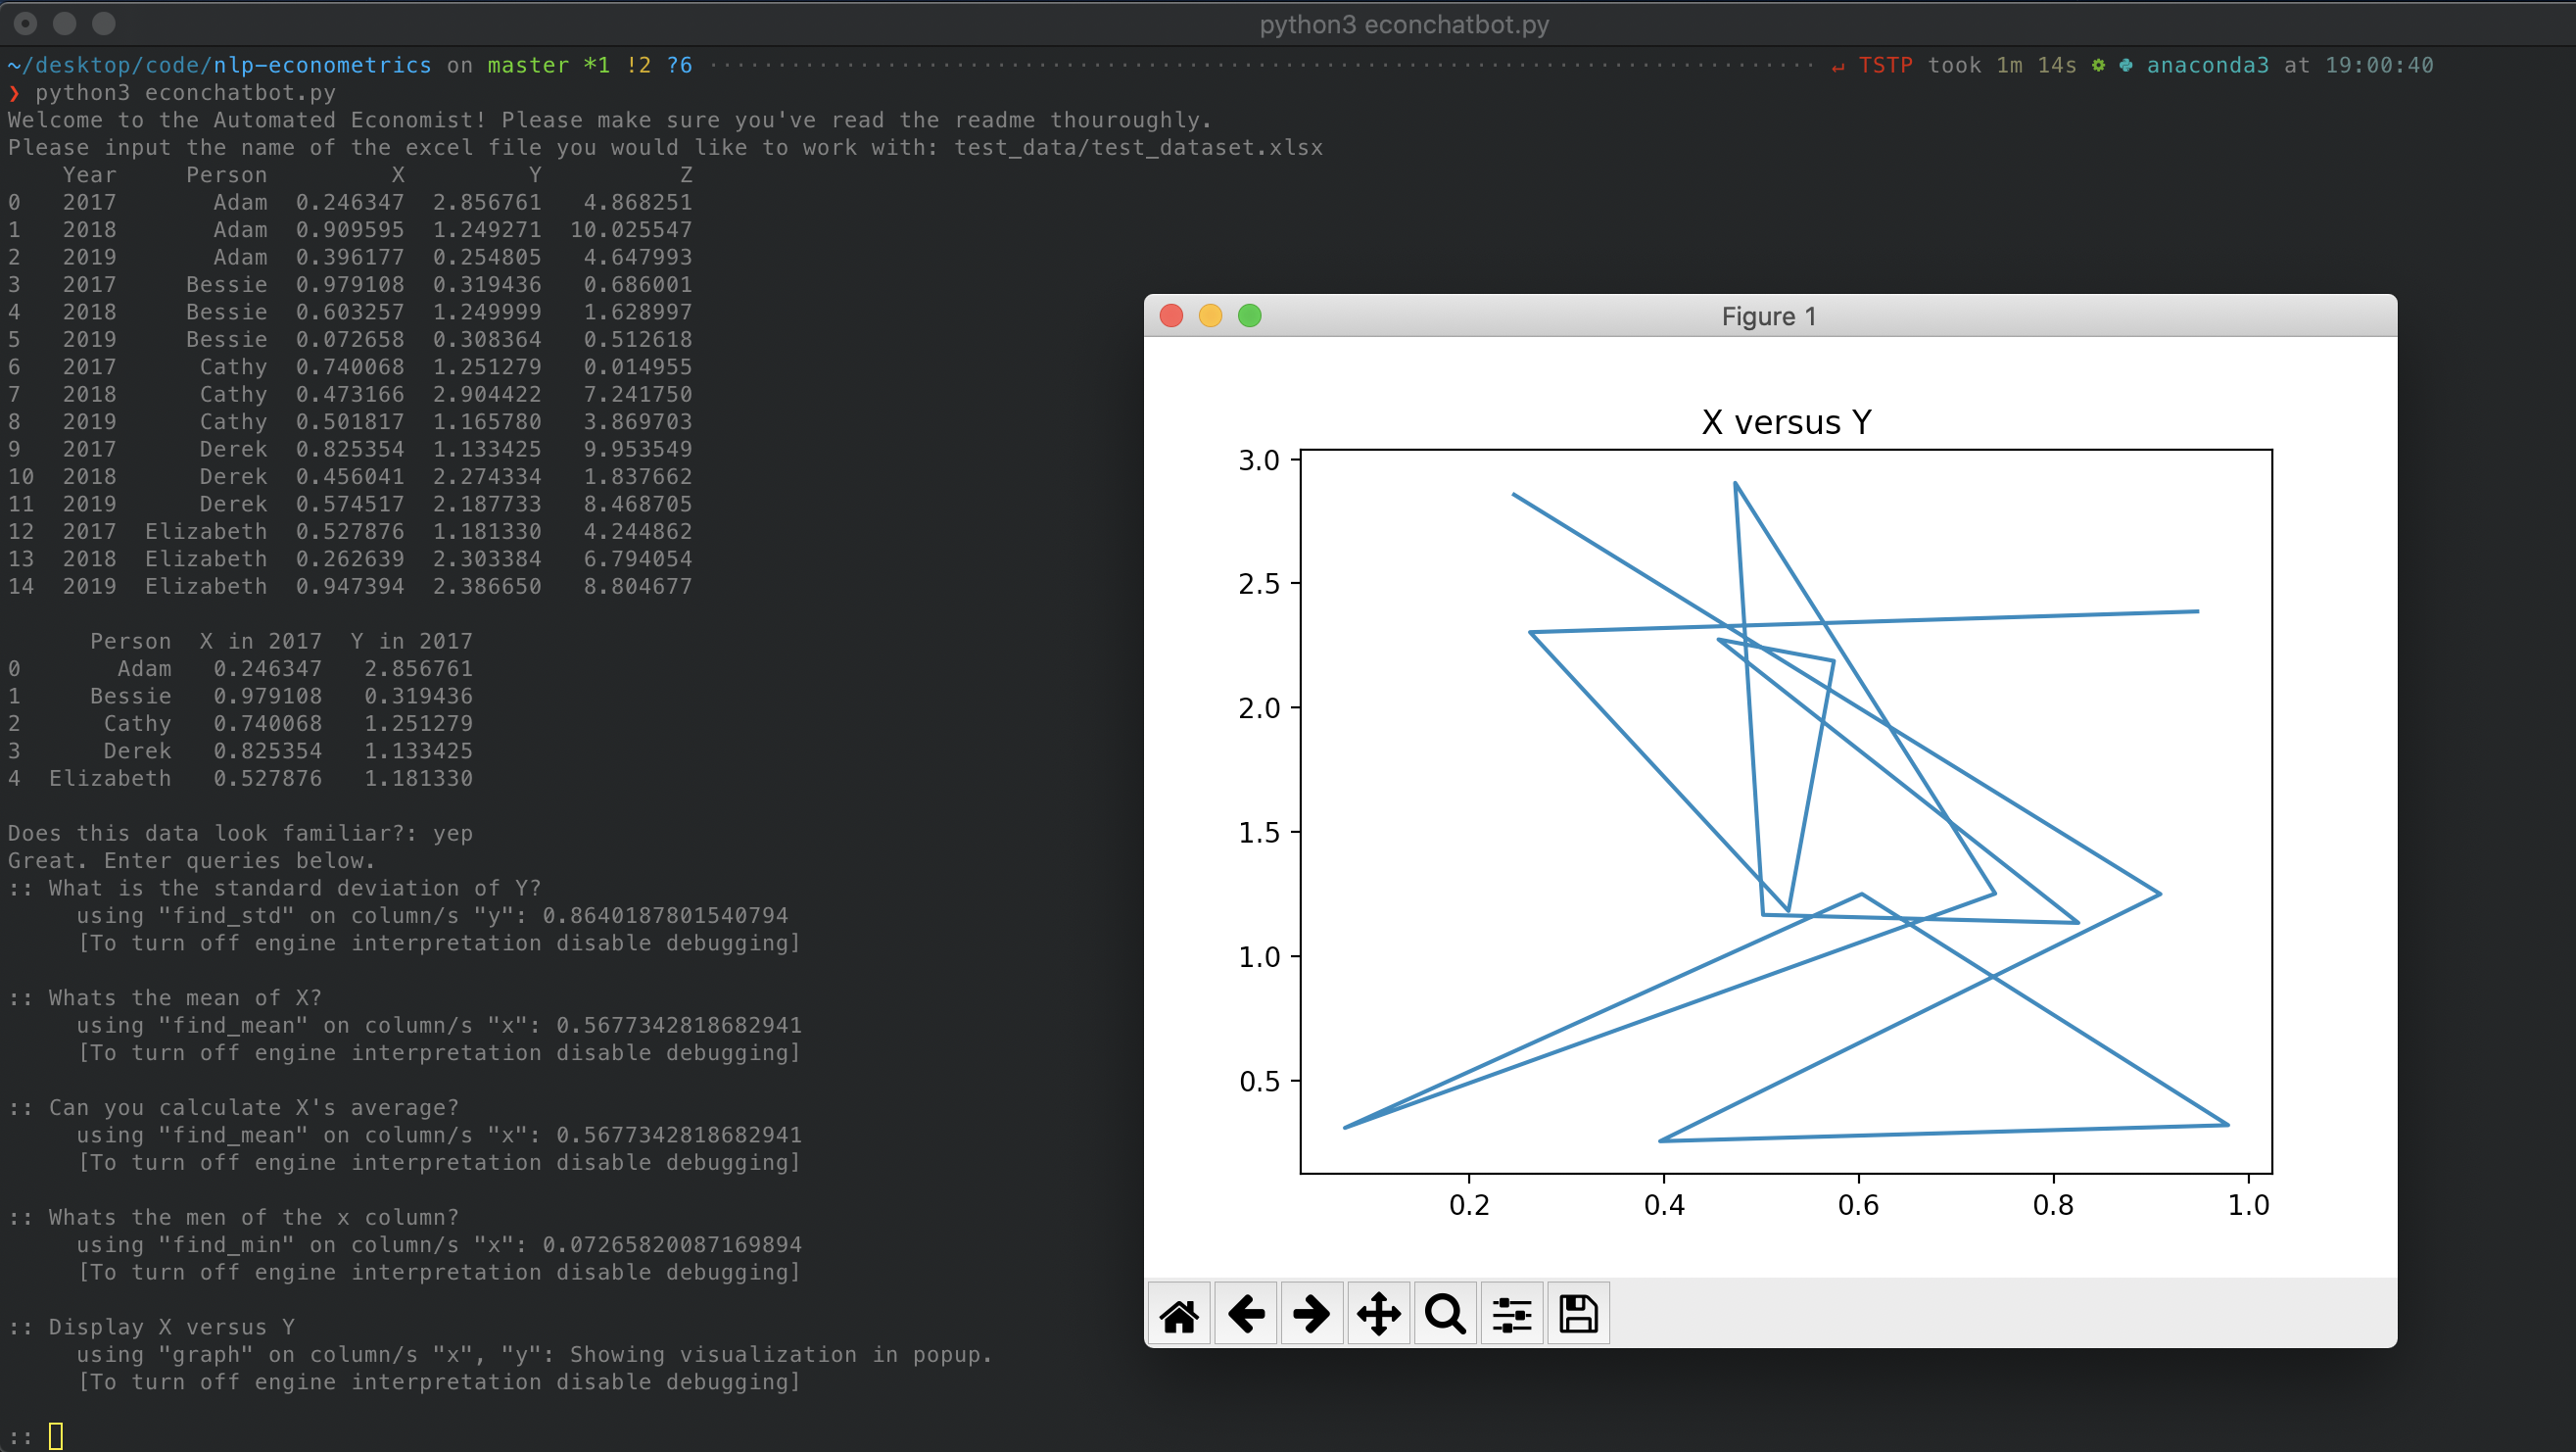
\includegraphics[width=1\linewidth]{imgs/screenshot.jpeg}
\caption{Example usage of our client.}
\label{fig:bot}
\end{figure}






\subsection{Progress So Far}
\begin{enumerate}
\item Working library for reading, writing, and storing xlsx data.
\item Class for automated reasoning about unseen data. 
\begin{itemize}
\item Reasons about column types. Assigns logical relationships between columns and assigns semantic meaning to data. (For example, reasoning that a numeric column is actually a date or that a string column is actually symbolic of a geometric location. Both of these are very important for answering queries that presume a knowledge of the dataset structure.)
\end{itemize}
\item Basic NLP Question parser using logical question parsing and levenshtein string-distance  and log-likelihood measures for deciphering uncleen queries. 
\begin{itemize}
\item As the point of the software is to be able to help untrained individuals, we would like our engine to be as "un-picky" as possible when it comes to question formats. Currently, our system is adept at handling misspellings, synonyms and the like when dealing with queries.
\end{itemize}
\item  Library of common statistical functions used in econometric analysis.
\item Basic CLI for using our application.
\begin{itemize}
\item Figure \ref{fig:bot} shows an example use of our program where the engine gets most queries right, but one incorrectly.
\end{itemize}
\end{enumerate}
\subsection{Plan of Attack}
Plan for the rest of the semester.
\begin{itemize}
\item Create an application (rather than CLI) for interacting with our engine.
\item Uitilize SEMPRE (a third party tool for semantic parsing) to augment our query parsing and handling.
\item Use Mechanichal Turk to generate lists of queries in order to continue to train our parsing tool.
\item Use a handful of econ students to test our client.
\begin{itemize}
\item We have 10 students who have volunteered to use our client.
\item This will help us in a number of ways: (1) it will provide us with more querying data for training. (2) Provide feedback for the use and feel of the application. (3) Users will be able to suggest and add their own econometric methods,.

\end{itemize}
\item Continue to expand usable statistical methods and tools for querying data.
\item Host a database for storing previous queries for online learning.
\end{itemize}




\bstctlcite{bstctl:etal, bstctl:nodash, bstctl:simpurl}
\bibliographystyle{IEEEtranS}
\bibliography{references}

\end{document}

